
\begin{figure*}
        \centering

        \begin{subfigure}[b]{0.4\textwidth}
                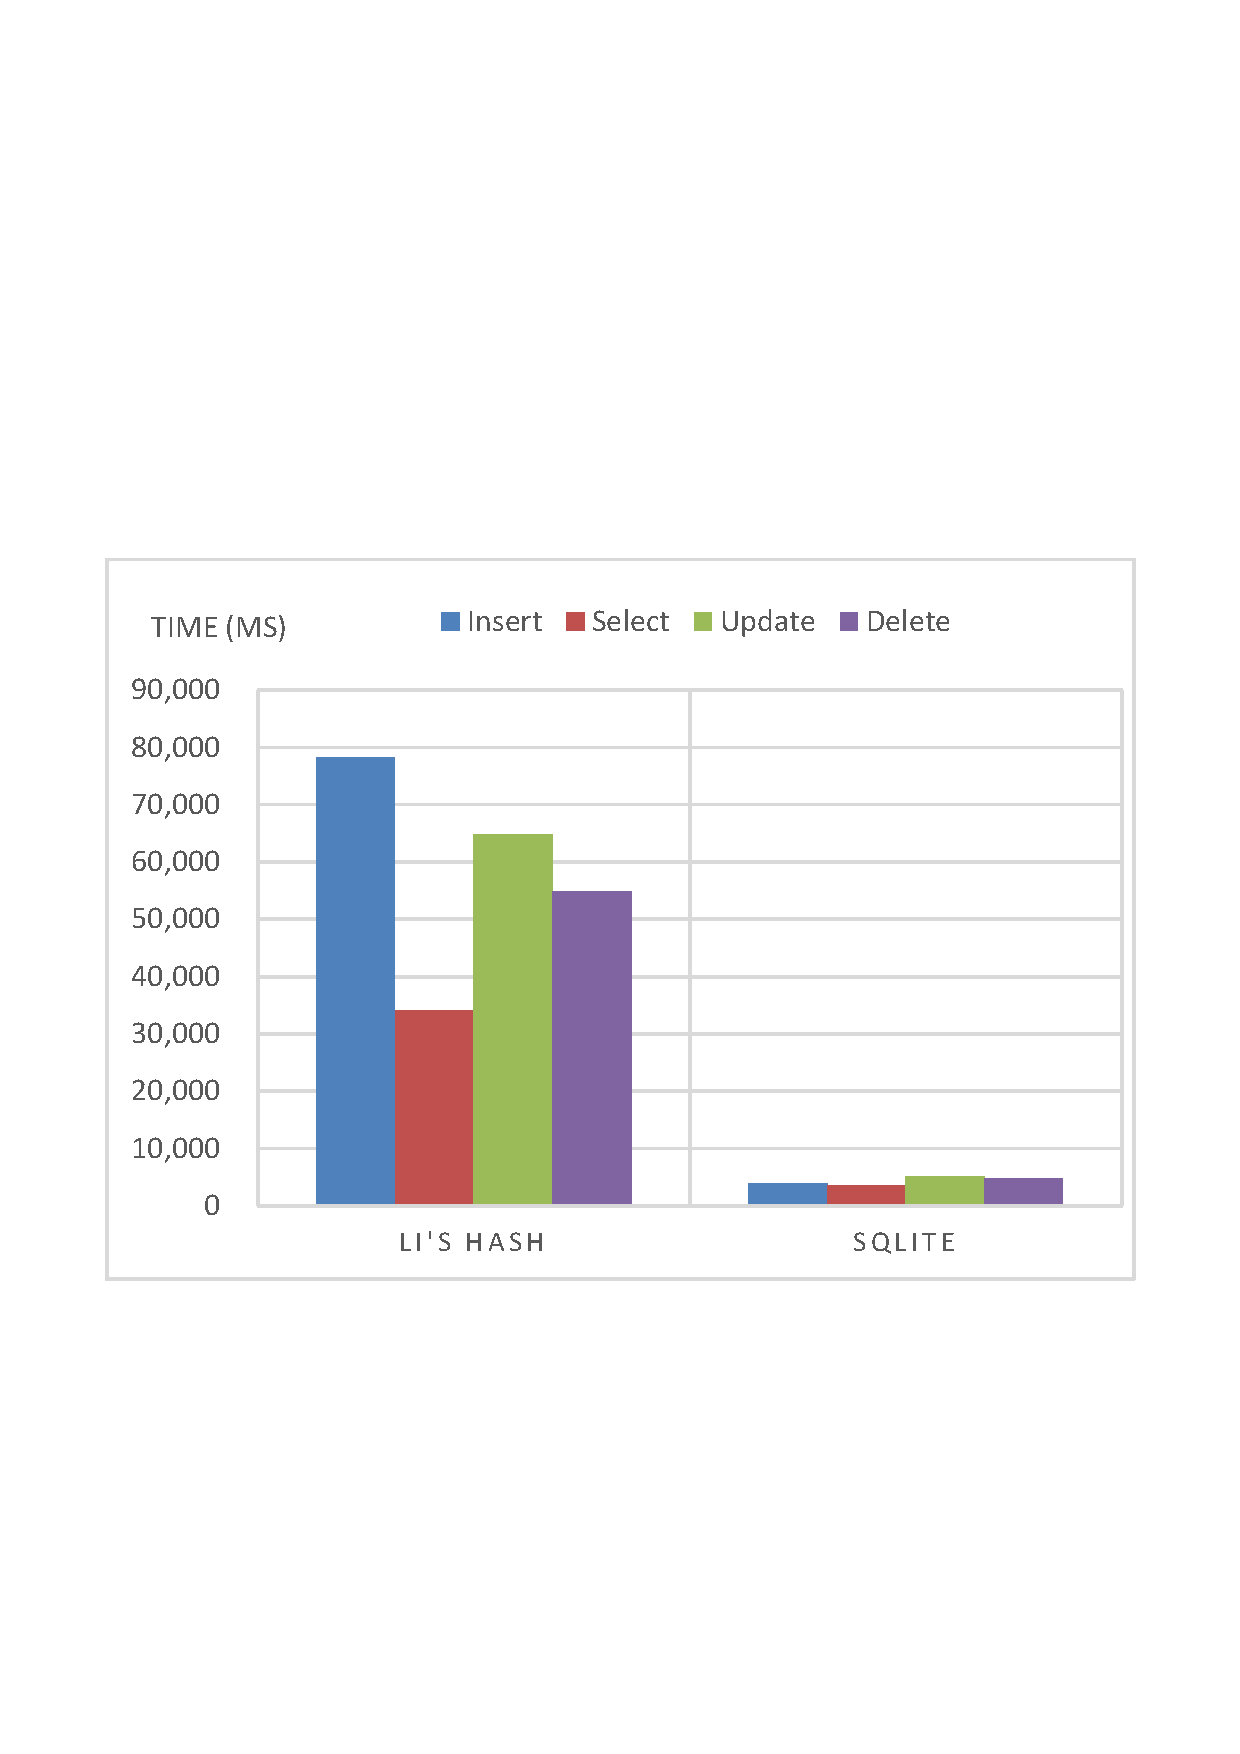
\includegraphics[width=\textwidth]{./performance/result/index-layer/image/100only/string1.pdf}
                \caption{STRING type}
                \label{fig:performance:result:index-layer:insert:boolean}
        \end{subfigure}%
        ~ %add desired spacing between images, e. g. ~, \quad, \qquad etc.
          %(or a blank line to force the subfigure onto a new line)
        \begin{subfigure}[b]{0.4\textwidth}
                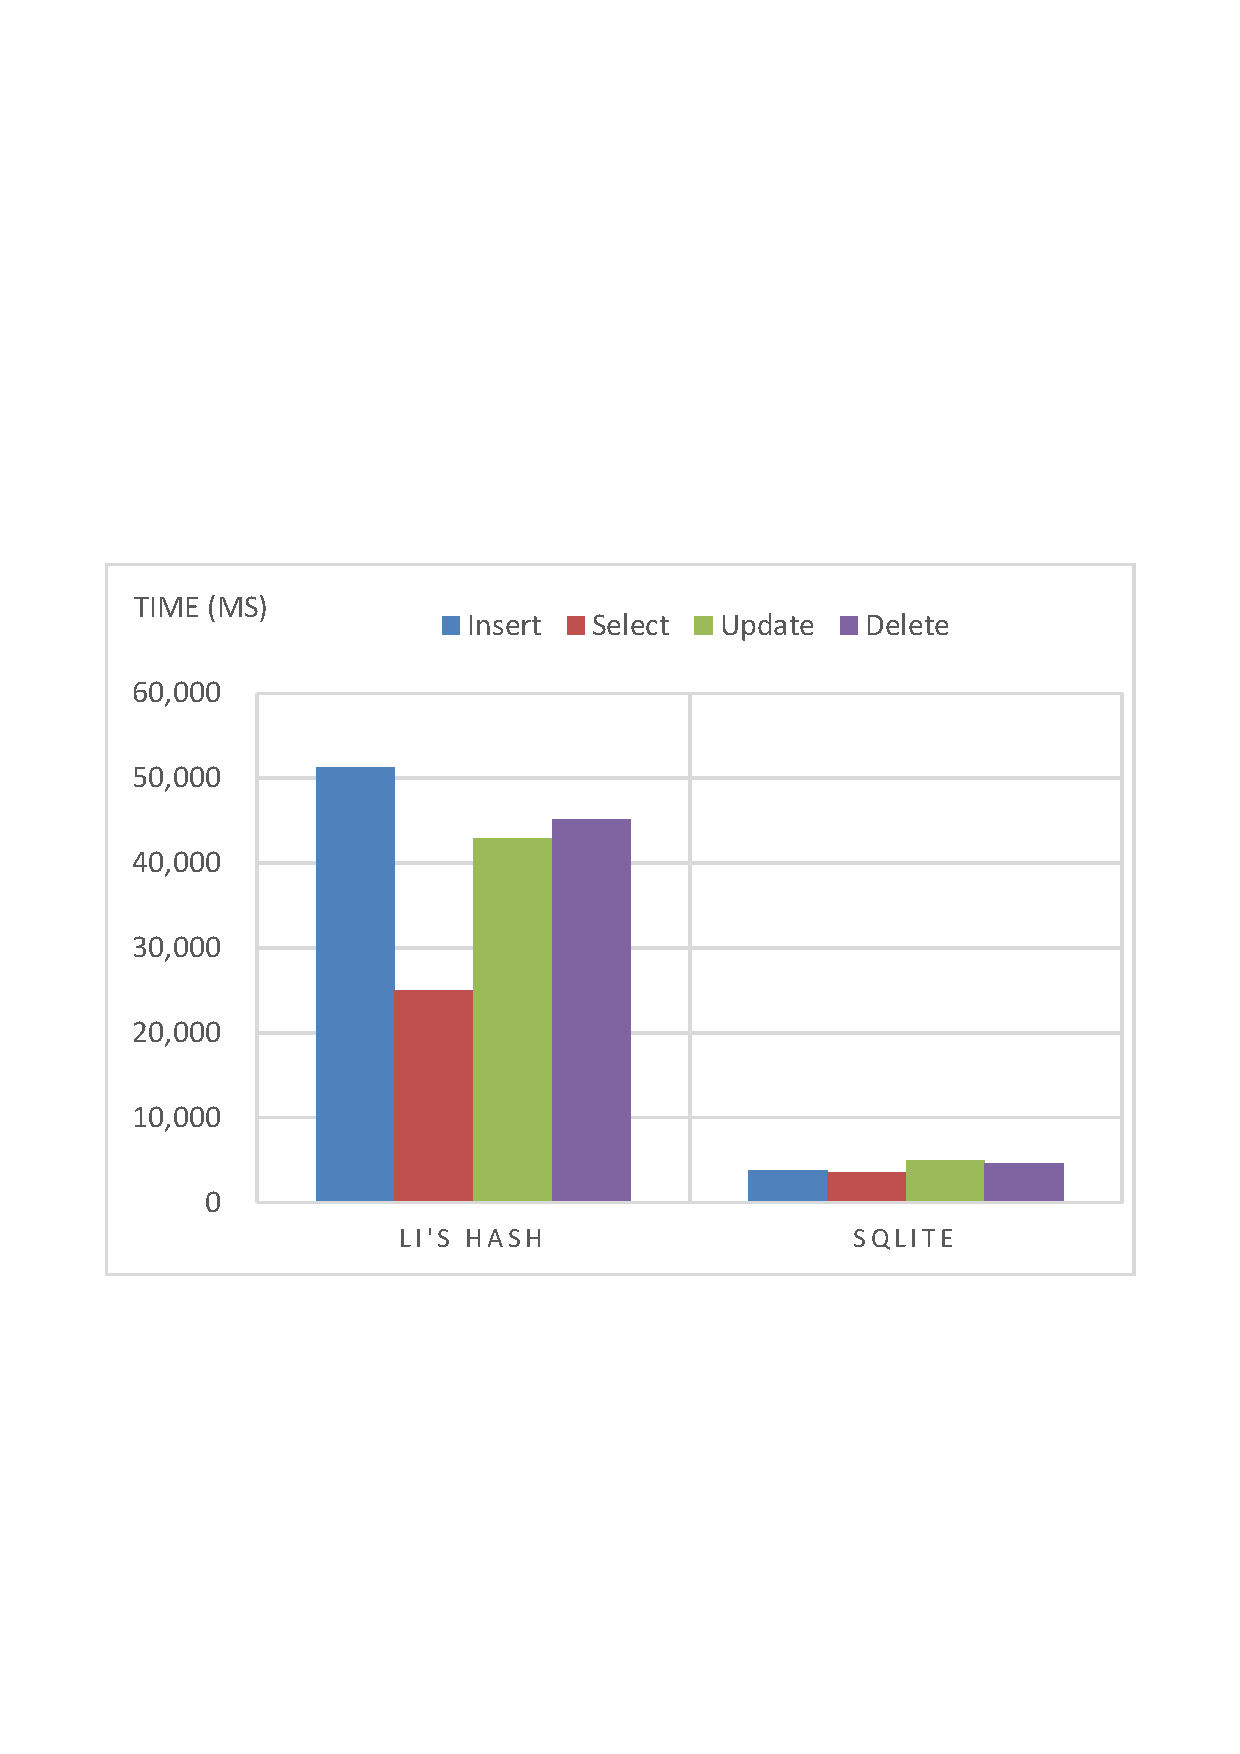
\includegraphics[width=\textwidth]{./performance/result/index-layer/image/100only/boolean1.pdf}
                \caption{BOOLEAN type}
                \label{fig:performance:result:index-layer:insert:int}
        \end{subfigure}

        \begin{subfigure}[b]{0.4\textwidth}
                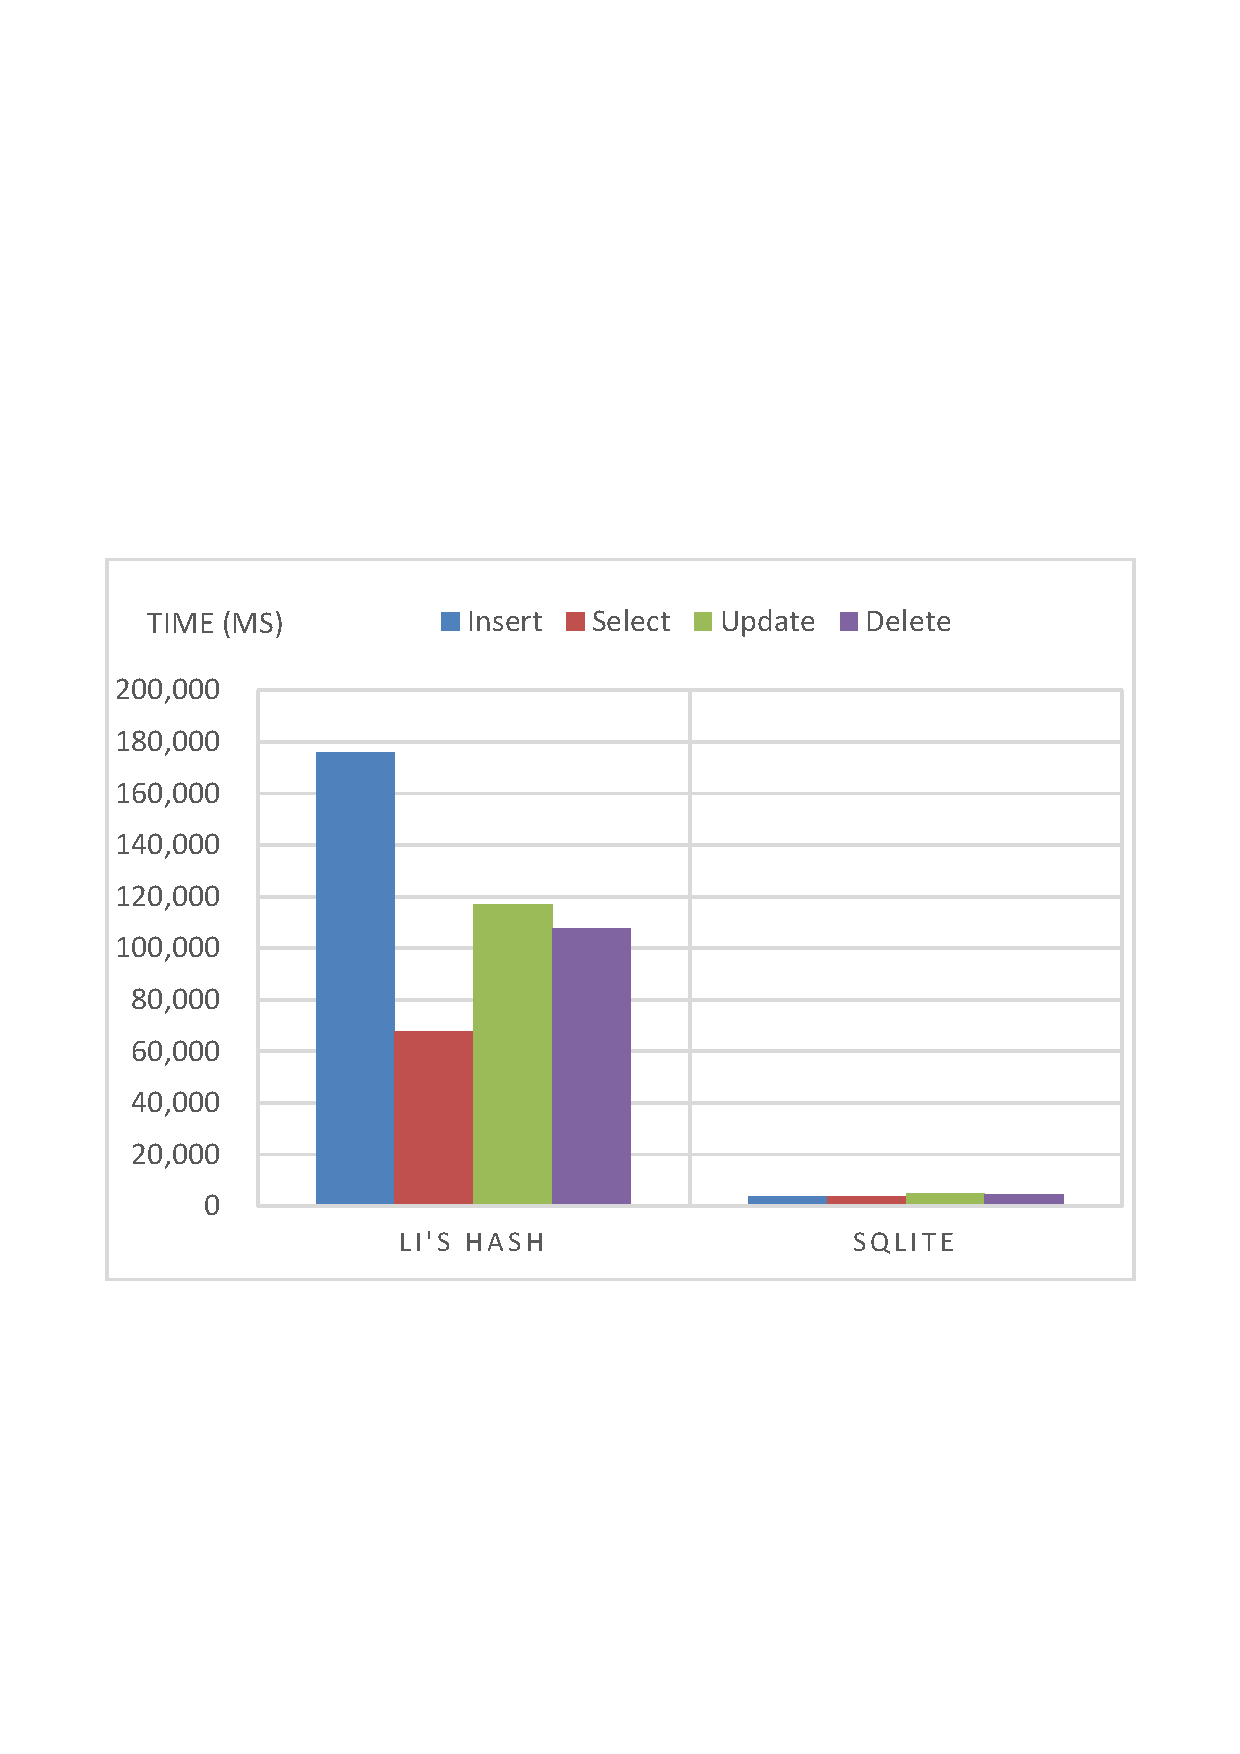
\includegraphics[width=\textwidth]{./performance/result/index-layer/image/100only/integer1.pdf}
                \caption{INTEGER type}
                \label{fig:performance:result:index-layer:insert:real}
        \end{subfigure}
        ~ %add desired spacing between images, e. g. ~, \quad, \qquad etc.
          %(or a blank line to force the subfigure onto a new line)
        \begin{subfigure}[b]{0.4\textwidth}
                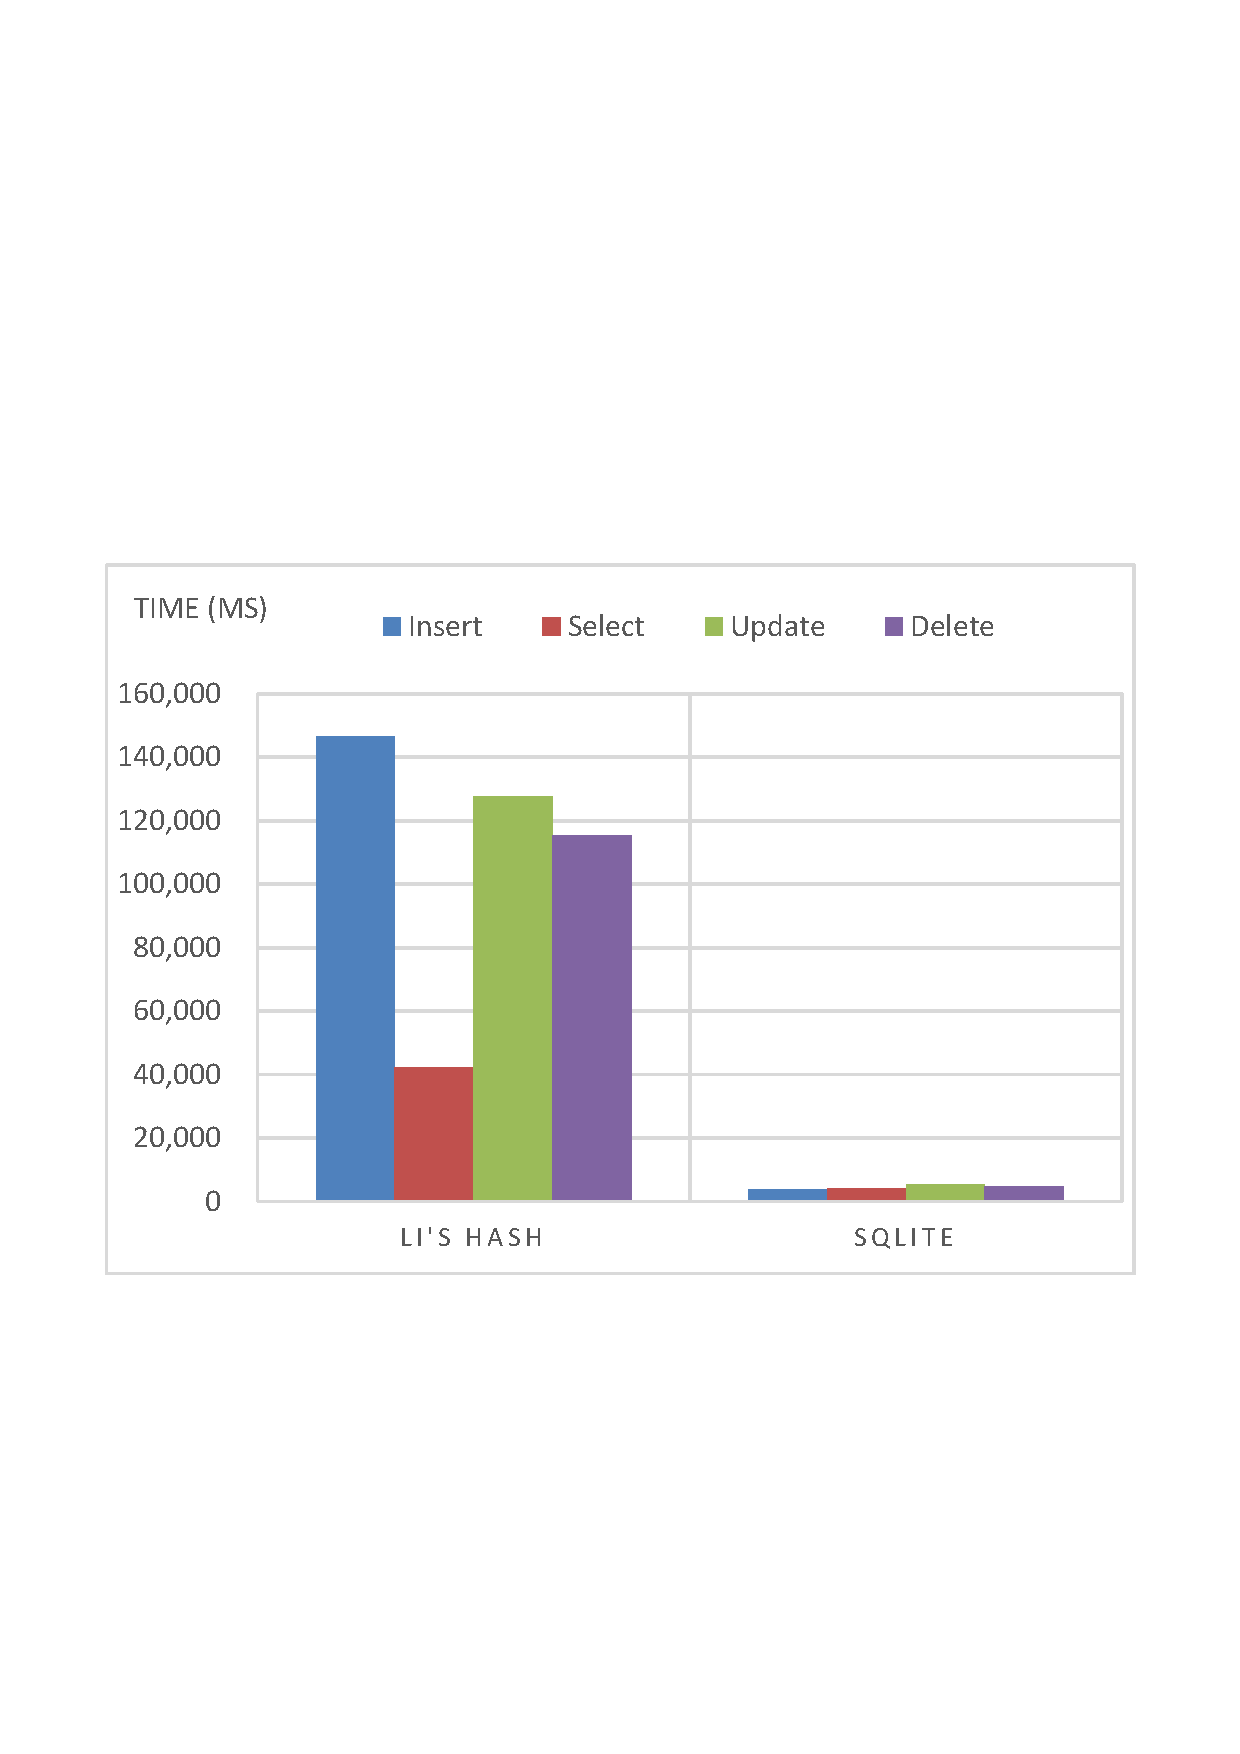
\includegraphics[width=\textwidth]{./performance/result/index-layer/image/100only/real1.pdf}
                \caption{REAL type}
                \label{fig:performance:result:index-layer:insert:string}
        \end{subfigure}

        \caption{Performance on index layer}
        \label{fig:performance:result:index-layer}
\end{figure*}

